\documentclass[yuxi]{../template/Report}%方括号内写yuxi即生成预习报告\documentclass[yuxi]{../template/Report}
\settemplatedir{../template/}%设置模板路径
\usepackage{enumitem}
\exname{} %实验名称
\extable{} %实验桌号
\instructor{} %指导教师
\class{} %班级
\name{} %姓名
\stuid{} %学号

\nyear{} %年
\nmonth{} %月
\nday{} %日
\nweekday{} %星期几,e.g. \nweekday{三}
\daypart{}%上午/下午

\redate{} %如有实验补做,补做日期
\resitu{} %情况说明:

\begin{document}
\maketitle%输出封面

\section{预习报告(10分)}
(注:将已经写好的“物理实验预习报告”内容拷贝过来)
\subsection{实验综述(5分)}
(自述实验现象、实验原理和实验方法,包括必要的光路图、电路图、公式等。不超过500字。)
\subsubsection{反射法测量三棱镜顶角}\label{func1}
用一束平行光入射到三棱镜的棱角,如\cref{fig:fig1},光线1经AB反射,光线2经AC反射,光线1和光线2的夹角为$\alpha$。实验中可用分光计的望远镜测量光线1和光线2的夹角,从而求出顶角$\angle A = \cfrac{\alpha}{2}$。
设两读数窗为I窗和II窗,当望远镜在右边时,读数分别为$\angle \text{右}_I, \angle \text{右}_{II}$;同理当望远镜在左边时,读数分别为$\angle \text{左}_I, \angle \text{左}_{II}$。则$\alpha_1 = (\angle \text{右}_I - \angle \text{左}_I)$,
$\alpha_2 = (\angle \text{右}_{II} - \angle \text{左}_{II})$。
为消除仪器的偏心差,取$\alpha = \cfrac{\alpha_1 + \alpha_2}{2}$,则顶角$\angle A = \cfrac{\alpha}{2}$。
即$\angle A = \cfrac{\left|\angle \text{右}_I - \angle \text{左}_I\right| + \left|\angle \text{右}_{II} - \angle \text{左}_{II}\right|}{4}$。
\begin{figure}[H]
    \centering
    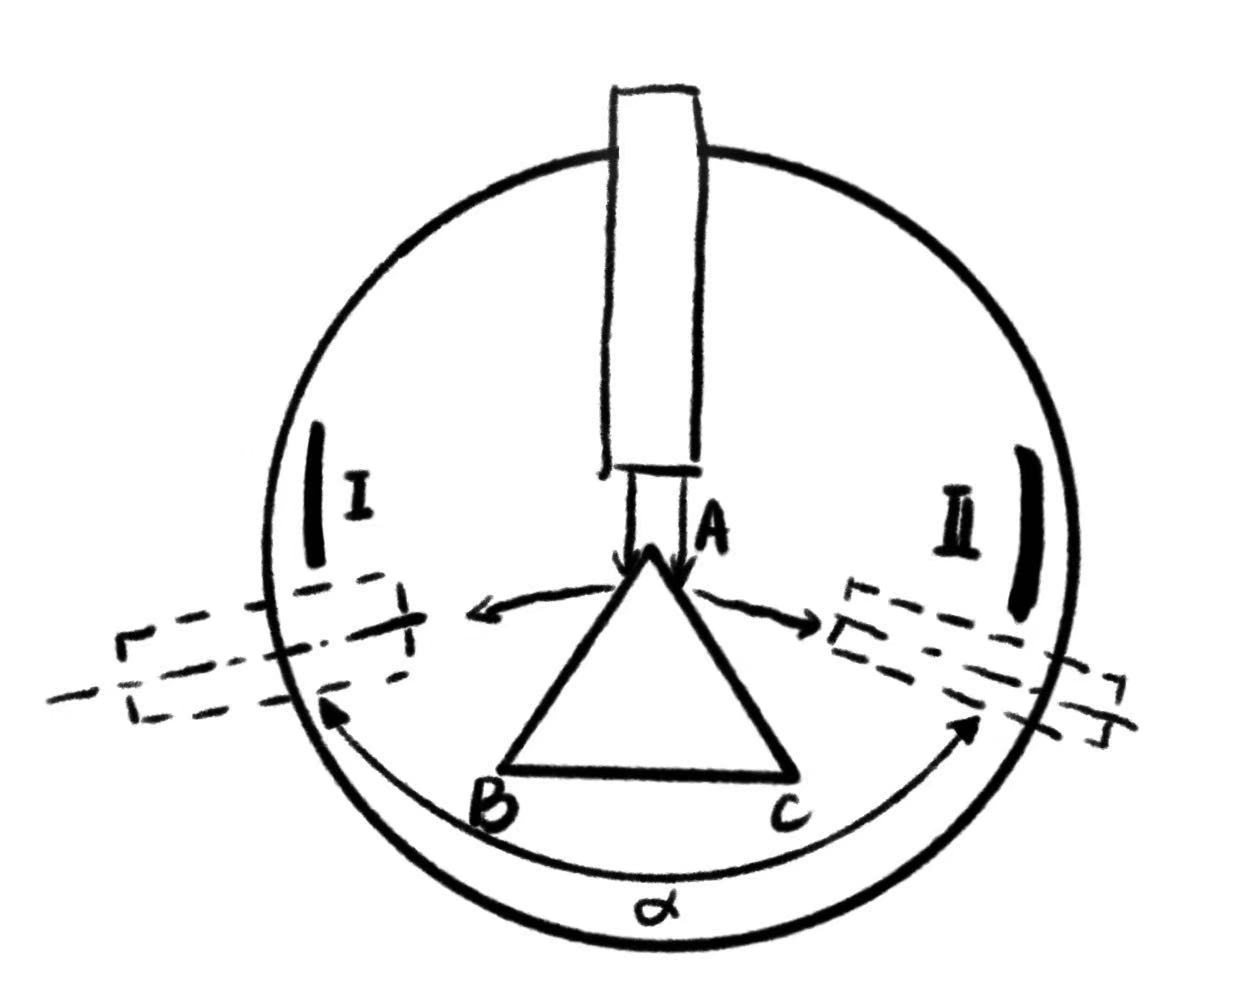
\includegraphics[width=0.5\textwidth]{反射法.jpg}
    \caption{反射法测量三棱镜顶角示意图}
    \label{fig:fig1}
\end{figure}
\subsubsection{自准直法}
在载物平台上放一镜面要垂直于望远镜光轴的平面反射镜。
调节亮十字与物镜间距离(即调焦),如果亮十字恰好处于物镜焦平面上,则亮十字上任意一点经物镜变为平行光。
该平行光由反射镜反射回来,经物镜后所成亮十字像应准确地处在亮十字所在平面上(如\cref{fig:fig2}所示)。
此时望远镜已调焦无穷远了。这种调焦方法称为自准直法。
\begin{figure}[H]
    \centering
    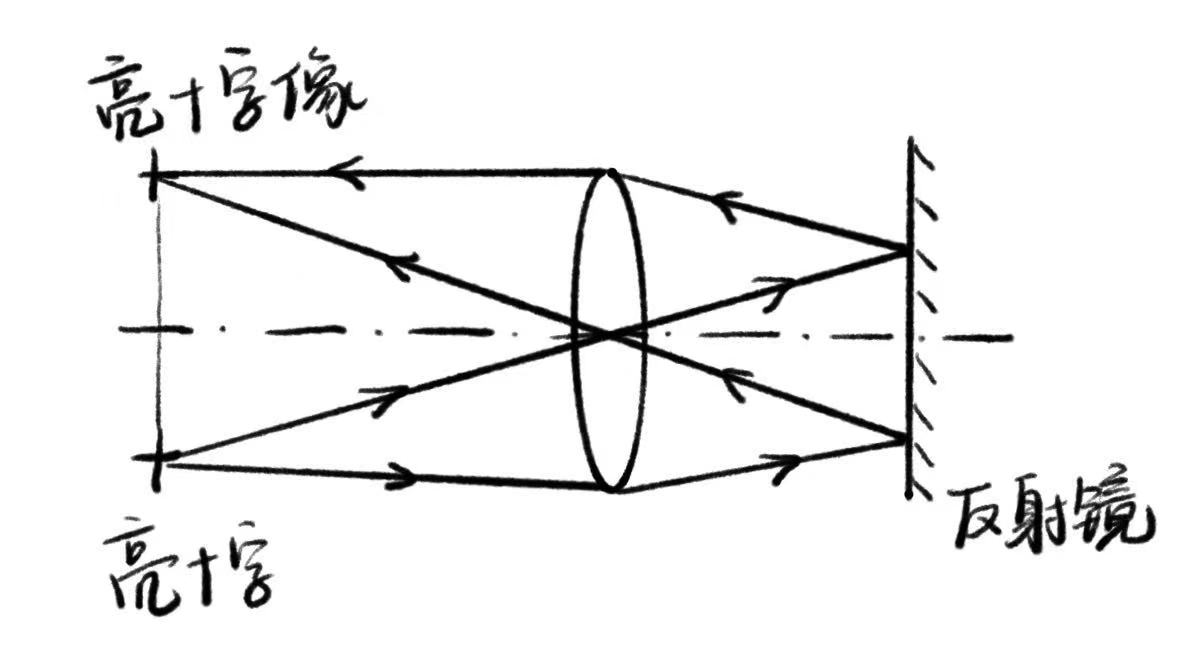
\includegraphics[width=0.5\textwidth]{自准直法.jpg}
    \caption{自准直法示意图}
    \label{fig:fig2}
\end{figure}
\subsection{实验重点(3分)}
(简述本实验的学习重点,不超过100字。)
\begin{enumerate}[left = 2em]
    \item 了解分光计的结构
    \item 学会正确的分光计调节和使用方法
    \item 利用分光计测量三棱镜顶角
\end{enumerate}
\subsection{实验难点(2分)}
(简述本实验的实现难点,不超过100字。)
\begin{enumerate}[left = 2em]
    \item \textbf{得到平行入射光:}必须精确地将平行光管调整好,确保从其出射的光线是平行光。任何发散或会聚的光都会引入测量误差。

    \item \textbf{望远镜的调焦:}将望远镜调焦至无穷远,使其能够准确接收并聚焦平行光。如果望远镜的焦距设置不准确,则无法清晰地观察到目标光束或谱线,导致读数困难和误差。

    \item \textbf{系统轴线的严格对准:}需要使平行光管的光轴与望远镜的光轴共轴或平行,并且这两者都必须垂直于分光计的中心轴。倾斜或偏离都可能会使光路几何发生改变,从而影响偏转角的准确测量。
\end{enumerate}
\begin{fullreportonly}
\section{原始数据(20分)}
(将有老师签名的“自备数据记录草稿纸”的扫描或手机拍摄图粘贴在下方,完整保留姓名,学号,教师签字和日期。)

\section{结果与分析(60分)}
\subsection{数据处理与结果(30分)}
(列出数据表格、选择适合的数据处理方法、写出测量或计算结果。)

\subsection{误差分析(20分)}
(运用测量误差、相对误差或不确定度等分析实验结果,写出完整的结果表达式,并分析误差原因。)

\subsection{实验探讨(10分)}
(对实验内容、现象和过程的小结,不超过100字。)

\section{思考题(10分)}
(解答教材或讲义或老师布置的思考题,请先写题干,再作答。)
\end{fullreportonly}
\insertnotes
\end{document}